% !TeX program = xelatex
% !TeX encoding = UTF-8
\documentclass{MathorCupmodeling}
\usepackage{mwe,color,float}
\usepackage[linesnumbered,ruled]{algorithm2e}
\usepackage{setspace}
\extrafloats{100}
\bianhao{MCB2201112}
\tihao{B}
\timu{\textbf{基于多模型调参优化的Stacking用户评分预测集成学习}}
\keyword{影响程度量化分析;特征工程;Stacking集成学习;评分预测;可视化评估}
\begin{document}
	\begin{abstract}
		这里是摘要
	\end{abstract}

	\pagestyle{empty}
	\tableofcontents
	\newpage
	\pagestyle{fancy}

	\setcounter{page}{1}
	\section{问题的提出}
	\subsection{问题背景}
	随着移动通信技术的迅猛发展和网络工程的不断建设,在信息透明、产品同质化的今天,提升语音通话及网络服务的质量,满足用户对高质量语音通话、网络服务的需求显得尤为重要。由于当今用户数量的不断增多、用户需求不断提高、运营商业务不断广泛化,因此点对点、传统方法解决问题逐渐困难化。而现在有来自移动通信集团北京分公司根据用户对语音业务及上网业务的满意度进行的评分及相关影响因素的数据,我们需要对其进行分析、建立相关数学模型,以便从数据中心获得有效信息,更高效地提升服务质量,为客户提供更好的服务。
	\subsection{问题要求}
	\begin{itemize}
		\item 初赛要求:
		\begin{itemize}
			\item \textbf{问题一}:研究并量化分析影响用户对语音及上网业务满意度的主要因素;
			\item \textbf{问题二}:建立基于影响用户评分影响因素的数学模型,并依据附件3、4中相关因素对其评分进行预测,并解释预测评分的合理性。
		\end{itemize}
		\item 复赛要求:
		\begin{itemize}
			\item \textbf{问题一}:结合初赛的分析、研究结果,分析用户对语音及上网业务的评分高低,并得出高分组与低分组的特征;同时对客户评分的合理性进行分析,筛选出评分合理的客户数据,并利用新的数据集重新建立预测模型,再对附件3、4中评分进行预测;
			\item \textbf{问题二}:依据初赛及复赛的分析结果,设计一份不超过一页纸的非技术报告,并将发现及建议提供给中国移动北京公司。
		\end{itemize}
	\end{itemize}

	\section{问题的分析}
	\subsection{问题的整体分析}
	该题是一个关于移动用户对语音及上网业务体验评分的数据分析、预测类问题。

	\textbf{从分析目的看},本题需要结合初赛的分析、研究结果,对数据集进行再分析,分析评分高分组与低分组的各自特征,对原数据集进行重采样,进行更深层次的分析。同时需要对用户的评分进行预测及研究,为运营商提供参考,从而提升用户语音及上网的优质体验。因此本题主要需完成两方面任务:{\heiti 其一},结合初赛的分析、研究结果,分析用户对语音及上网业务的评分高低,并得出高分组与低分组的特征;同时对客户评分的合理性进行分析,筛选出评分合理的客户数据,并利用新的数据集重新建立预测模型,再对附件3、4中评分进行预测;{\heiti 其二},依据初赛及复赛的分析结果,设计一份不超过一页纸的非技术报告,并将发现及建议提供给中国移动北京公司。

	\textbf{从数据来源、特征看},本题的数据来源于北京移动用户的语音与上网业务评分数据,数据包括用户对语音业务下“语音通话整体满意度”“网络覆盖与信号强度”“语音通话清晰度”“语音通话稳定性”,上网业务下“手机上网整体满意度”“网络覆盖与信号强度”“手机上网速度”“手机上网稳定性”方面的评分,以及相关的影响评分的因素。评分数据具有主观性,影响因素数据具有高维、多样、标准体系不一致、量纲不一致等特点,且数据量较大。因此,本题数据相对特殊且复杂,需要对数据进行一定的预处理,以便于后续的分析。
	
	\textbf{从模型的选择看},本题数据量较大、维度较高,且分析目的是分析影响用户评分的主要因素,并对用户的评分进行预测及研究。本文将评分视为多分类,且评分具有一定主观性、分类种类多,因此,在模型的选择上,本文结合多种分类预测模型,构建集成学习模型,尽可能多地学习到用户评分特点,提升模型的准确性、稳健性及可泛化性能。

	\textbf{从软件的选择看},本题为数据类型,且需要进行大量的数据分析、预测等,因此我们选择Python Jupyter对问题进行求解,其交互式的编程范式,方便且高效。

	\subsection{初赛总结}
	{\heiti 针对问题一},主要需要对用户语音及上网业务评分影响因素的程度进行量化分析。我们首先对数据集进行统一处理,包括:\textbf{初步剔除相关列数据}、\textbf{学习数据与预测数据指标一致化}、\textbf{指标规范化}、\textbf{空缺值处理}、\textbf{标签编码}、\textbf{特征构造}、\textbf{数据标准化}、\textbf{学习数据与预测数据一致化}、\textbf{学习数据训练集与测试集划分}。之后在处理好的数据集上建立\textbf{熵权法}、\textbf{灰色关联度分析}、\textbf{随机森林分类}模型,多方面综合考虑,量化分析各影响因素对评分的影响程度,并依此来确定影响用户两项业务满意度的主要因素。量化结果接近于实际生活,效果良好,且可为后续问题奠定基础。
	
	{\heiti 针对问题二},主要需要根据已有影响因素对用户的评分进行预测,并解释预测的合理性。我们首先结合问题一量化结果以及建立\textbf{主成分分析}模型,对数据\textbf{累计方差}进行解释,确定特征个数;之后建立\textbf{XGBoost模型},并得出各影响因素的重要性,与随机森林模型结合分析,确定特征的选择;再建立\textbf{KNN}、\textbf{SVM}、\textbf{LightGBM}以及\textbf{多分类逻辑回归模型},对数据进行学习分析;随后,对各个模型进行\textbf{超参数调优},模型准确率均有大幅度提升,如随机森林\textbf{较原先提升了}$\boldsymbol{11.69\%}$,\textbf{最高提升较原先可达到}$\boldsymbol{14.25\%}$,效果良好。再者,以模型的准确率、平均绝对误差、均方误差为标准,选择表现较优的模型作为\textbf{Stacking集成学习}的基模型,同时选择余下的一个模型作为第二层模型,在提升准确率的同时,避免过拟合。同时对其采用\textbf{五折交叉验证},验证其\textbf{稳健性}。Stacking集成学习结果符合预期效果,且明显优于单一模型。在保证准确率的同时,预测的平均绝对误差、均方误差\textbf{均有一定优化},同时我们还注重结果的可解释性及模型的现实意义。最后,我们进行\textbf{可视化分析},绘制原始数据及预测数据评分人数\textbf{南丁格尔玫瑰图},查看数据分布,绘制模型的\textbf{混淆矩阵热力图}、\textbf{分类报告}、\textbf{ROC/AUC曲线},多方面评估模型效果及解释模型的合理性。综合上述分析,可以确认模型效果良好,具有良好的稳健性、泛化能力。
	
	{\heiti 最后},我们还对所建立的模型的优缺点进行了中肯的评价、提出了模型的改进措施以及对模型进行了一定推广。

	{\heiti 因此},\textbf{本复赛解决方案建立在初赛的分析及结果基础之上},且重要部分本文会再提及。

	\subsection{问题一的分析}
	问题一的核心目的在于\textbf{对原数据集进行重采样,并进行更深层次的分析}。对于主观性因素过强的用户评分数据,为尽可能提升预测的准确率,我们需要先筛选出高分组及低分组用户,对其行为特征进行分析,筛选出评分合理的用户,依此重新建立分类预测模型,提升移动公司对用户对各项业务的满意程度的把握程度,从而更好地解决现存问题,为用户提供更优质服务。
	\subsection{问题二的分析}
	问题二的核心目的在于\textbf{为移动公司撰写一份非技术性报告,为其提供合理性建议,从而为客户提供更好的服务}。
	\section{符号说明}
	\begin{center}
		\scalebox{0.92}{
		\begin{tabularx}{0.7\textwidth}{c@{\hspace{1pc}}|@{\hspace{2pc}}X}
			\Xhline{0.08em}
			符号 & \multicolumn{1}{c}{符号说明}\\
			\Xhline{0.05em}
			$\mu$ & 样本平均值\\
			$\sigma$ & 样本方差\\
			$x_{\mathrm{standard}}$ & 经过标准化后的数据\\
			$R\left(x\right)_{m\times n}$ & 经过某项处理后的数据特征集\\
			$\rho$ & 皮尔逊相关系数\\
			$x'$ & 经过某项处理后的数据\\
			$Gini$ & 样本集合基尼系数\\
			$\hat{y}$ & 预测值\\
			$L^{\left(t\right)}$ & 目标函数\\
			$\Omega$ & 叶节点正则项惩罚系数\\
			$P$ & 某事件发生的概率\\
			$\omega$ & 权重\\
			\Xhline{0.08em}
		\end{tabularx}}
	\end{center}
	\section{模型的假设}
	本文对于模型的假设与初赛假设一致,如下:
	\begin{itemize}
		\item \textbf{假设一}:语音与上网业务的八项评分中,存在个别用户乱评、错评现象;
		\item \textbf{假设二}:除个别用户的部分评分外,其余所有数据真实且符合实际情况;
		\item \textbf{假设三}:用户评分还受到除附件中因素之外的因素的影响;
		\item \textbf{假设四}:给定的数据集可全面体现用户整体情况;
		\item \textbf{假设五}:对于同一业务,学习数据与预测数据的内在规律是一致的。
	\end{itemize}
	\section{模型的建立与求解}
	\subsection{相关准备工作}
	为方便、准确、高效解决问题,我们需要对数据进行预处理,其主要过程见\textcolor{blue}{\cref{fig:dataprepare}},包括:初步剔除相关列数据、学习数据与预测数据指标一致化、指标规范化、空缺值处理、标签编码、特征构造、标准化、学习数据与预测数据一致化、学习数据训练集与测试集划分。\textbf{本文后续的模型建立都在此基础之上}。上述过程与初赛大致相同,但本文对部分进行的合理地修改,以适应本题要求。
	\begin{figure}[H]
		\centerline{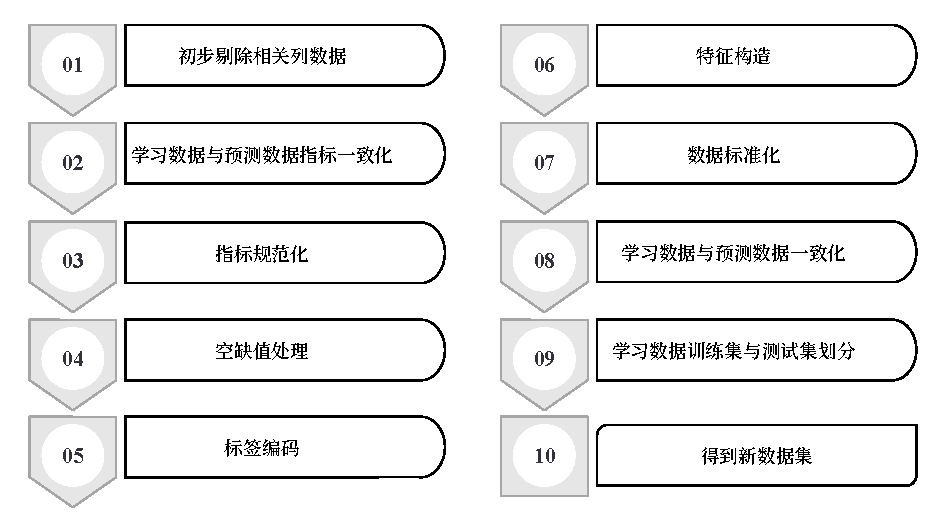
\includegraphics[scale=0.78]{数据的准备.pdf}}
		\caption{数据的准备主要过程}\label{fig:dataprepare}
	\end{figure}
	\subsubsection*{Step1 初步剔除相关列数据}
	由于“用户id”为连续编号,且与评分无任何关系,故本文将该列数据剔除;同时对于“用户描述”等文字性叙述指标,由于其均为文本,且描述特征难以提取,难以量化,本文将该列数据剔除,但为了获得客户相关描述,本文将绘制用户描述高频词汇云图;此外,对于“终端品牌类型”等多类别指标,由于其类别较多,量化后难以提取出有效信息,故也将其剔除,其余列暂时保留。
	\subsubsection*{Step2 学习数据与预测数据指标一致化}
	附件1与附件3为用户语音业务数据,但两表数据影响的因素存在不一致的现象,需要对指标取交集,确保两者一致,附件2与附件4同理。这里我们利用Python中集合set容器元素唯一性特征及pandas库,筛选出相同因素。而对于可能重合的指标,我们在下文也会进行一定处理。这样即可确保在学习数据上建立的模型依据的指标存在于预测数据集上,避免两者指标不一的情况。
	\subsubsection*{Step3 指标规范化}
	经过上述处理后,我们发现大部分影响因素为分类指标,其划分“是”“否”的字段不统一,故依据“附件5附件1、2、3、4的字段说明.xlsx”文件,本文对附件1、2、3、4中的分类指标进行规范化,记“是”类别为1,“否”类别为0,方便后续模型的建立。
	\subsubsection*{Step4 空缺值处理}
	在给定数据集中,部分空缺值可以依据附件5的解释进行填充。经过一定处理后,附件3与附件4中无空缺值,故本文对附件1与附件2中的空缺值进行分析与处理:
	\begin{itemize}
		\item \textbf{对于附件1}:据附件5解释进行填充后,还存在个别用户的空缺值,空缺值的列名为:“是否4G网络客户(本地剔除物联网)”“终端品牌”“是否5G网络客户”“客户星级标识”,且这些空缺值均在同一用户中出现,用户id分别为1573、1601、2326、2827、3265。附件1的空缺值有集中、个数少的特点,存有空缺值的用户仅有5个,占整体用户的$0.0920\%$,对于模型的建立影响较小,因此我们将这5行用户剔除。
		\item \textbf{对于附件2}:经过指标一致化后及初步数据空缺值的填补后,附件2中仅剩“终端品牌”列指标存在14个空缺值,根据该列数据其余特征,我们将这个14个空缺值以0填充。
	\end{itemize}
	\subsubsection*{Step5 标签编码}
	首先,对用户的评分进行编码,由于部分分类模型需要分类量值从0开始,因此,为方便后续集成学习等,本文将评分从$\left[1,10\right]$映射至$\left[0,9\right]$,且仍均为整数,即将评分减1。其次,对“终端品牌”“4\textbackslash{}5G用户”指标利用Python的sklearn库中的LabelEncoder进行标签编码。此外,对于“客户星级标识”指标,我们依据移动公司对客户星级标识的划分进行编码,编码值对应见\textcolor{blue}{\cref{tab:1}}。
	\begin{table}[htbp]
		\centering
		\caption{客户星级标识编码对应表}\label{tab:1}
		\scalebox{0.8}{
		\begin{tabular}{ccccccccc}
			\toprule
			未评级 & 准星 & 一星 & 二星 & 三星 & 银卡 & 金卡 & 白金卡 & 钻石卡 \\
			\midrule
			0 & 1 & 2 & 3 & 4 & 5 & 6 & 7 & 8 \\
			\bottomrule
		 \end{tabular}}
	\end{table}
	\subsubsection*{Step6 特征构造}
	观察并分析给定的数据,我们可以构造以下特征:
	\begin{itemize}
		\item \textbf{对于附件1与附件3}:
		\begin{itemize}
			\item 观察到附件1中有“家宽投诉”与“资费投诉”两项,而在附件3中有“是否投诉”一项,因此,我们在附件1中构造“是否投诉”一项。若“家宽投诉”与“资费投诉”均为0,则“是否投诉”记为0,否则记为1。并同时删去“家宽投诉”与“资费投诉”;
			\item 观察到附件1中有多个出现问题的场所,因此我们将每一用户出现问题的场所求和,构造“场所合计”,他们为“居民小区”“办公室”“高校”“商业街”“地铁”“农村”“高铁”“其他,请注明”;
			\item 观察到附件1中有多个类型的问题,因此我们将出现问题求和,构造出“出现问题问题合计”,他们为“手机没有信号”有信号无法拨通”“通话过程中突然中断”“通话中有杂音、听不清、断断续续”“串线”“通话过程中一方听不见”“其他,请注明.1”;
			\item 观察到附件1中“脱网次数”“mos质差次数”“未接通掉话次数”有相似特征,故将每一用户该三项数据求和,构造出“脱网次数、mos质差次数、未接通掉话次数合计”。
		\end{itemize}
		\item \textbf{对于附件2与附件4}:
		\begin{itemize}
			\item 观察到附件2中有多个出现问题的场所,构造出“出现问题场所或应用总”;
			\item 观察到附件2中“手机上网速度慢”“打游戏延时大”“显示有信号上不了网”“全部都卡顿”“全部游戏都卡顿”“手机支付较慢”“看视频卡顿”“上网过程中网络时断时续或时快时慢”“打开网页或APP图片慢”“全部网页或APP都慢”“下载速度慢”“网络信号差/没有信号”特征相似,故将每一用户对应的项目数据求和,构造出”网络卡速度慢延时大上不了网总“;
			\item 观察到附件2中“微信质差次数”以及“上网质差次数”均为质差量值,故将每一用户该二项数据求和,构造出“质差总”;
			\item 观察到附件2中的场所类别较多,故将场所求和,构造出“地点总”。
		\end{itemize}
	\end{itemize}
	\subsubsection*{Step7 数据标准化}
	该处标准化处理为\textbf{Z-score}方法,仅用于后续机器学习模型的使用。而在问题一的熵权法、灰色关联度分析中我们采用\textbf{Min-Max}方法,该方法在后文模型中会具体说明。

	对于某一列数据$x=\left[x_1,x_2,\cdots,x_m\right]^{\mathrm{T}}$,其平均值为
	\begin{equation}
		\mu=\frac{1}{m}\sum_{i=1}^{m}x_i \label{fmean}
	\end{equation}
	标准差为
	\begin{equation}
		\sigma=\sqrt{\frac{1}{m}\sum_{i=1}^{m}\left(x_i-\mu\right)^2} \label{fstd}
	\end{equation}
	则标准化后的数据为
	\begin{equation}
		\left(x_{\mathrm{standard}}\right)_i=\frac{x_i-\mu}{\sigma} \label{fstandardprocess}
	\end{equation}

	利用上述计算公式,我们对非分类指标进行处理,使得原数据经过处理后,其值聚集于0附近,即均值为0,标准差为1。这样处理,利于机器学习模型的建立、学习与预测,加快模型的收敛速度,并在一定程度上提升模型的准确性。同时该标准化处理方法适合当代嘈杂的大数据场景\textcolor{blue}{\cite{pstandard}}。因此对于大样本的数据,如出现部分异常值,使用该方法对最终结果影响较小。
	\subsubsection*{Step8 学习数据与预测数据一致化}
	经过上述几项处理后,我们还需要将附件1与附件3数据集一致化,包括指标一致化以及数据字段、分布排列一致化,从而保证对于需要预测的数据集附件3利用在附件1中建立的模型所利用到的数据集的一致性,避免造成数据的不一致,导致预测错误。本文对附件2与附件4进行上述相同的操作。
	\subsubsection*{Step9 学习数据训练集与测试集划分}
	为计算问题二中建立的模型的准确性等指标,需要在附件1与附件2中均划分训练集与测试集。对于语音业务划分训练集与测试集比例为8:2;而对于上网业务,其比例设为9:1。对于比例的设置,本文将在后文解释其合理性。且上述划分利用sklearn库中的train\_test\_split函数实现,且任意设定随机种子为2022,确保多次调试结果的一致性。该函数可确保划分的随机性,确保训练集与测试集数据分布规律大致相同。

	\subsection{问题一模型的建立与求解}
	对于问题一,我们综合用户评分箱线图、用户评分联合分布图,并结合初赛得出的各项因素重要性程度,对数据进行更深层次分析,筛选出评分合理的用户群体,并依据该数据建立多分类预测模型,预测未知评分的用户集体对于语音及上网业务的满意程度。
	\subsubsection{语音业务及上网业务数据分析}
	首先,我们绘制出用户对于语音及上网业务评分的箱线图,如\textcolor{blue}{\cref{fig:语音业务箱线图}}、\textcolor{blue}{\cref{fig:上网业务箱线图}}所示。
	\begin{figure}[H]
		\centering
		\begin{minipage}{0.48\linewidth}
			\centering
			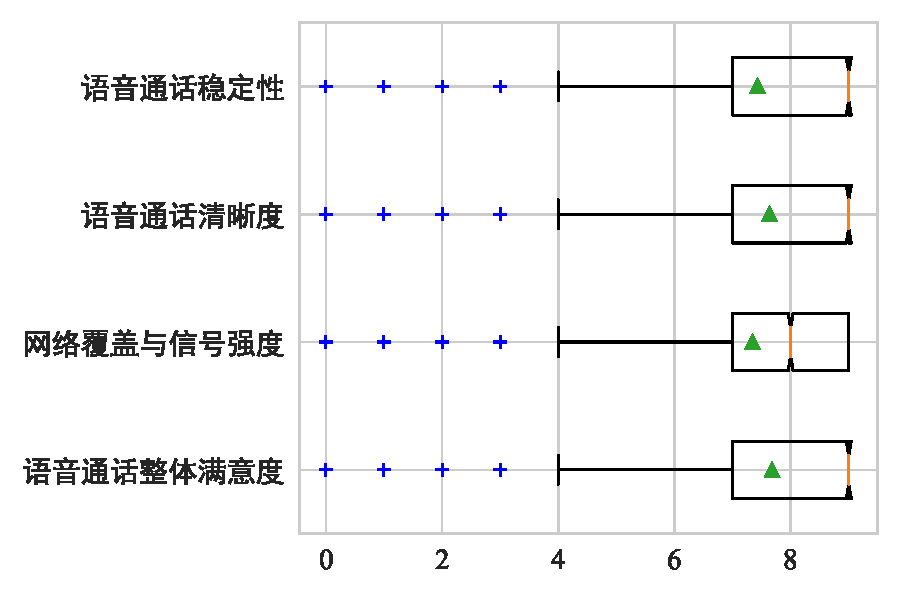
\includegraphics[width=1.0\linewidth]{[附件1][语音通话整体满意度、网络覆盖与信号强度、语音通话清晰度、语音通话稳定性]评分箱线图.pdf}
			\caption{语音业务用户四项评分箱线图}
			\label{fig:语音业务箱线图}
		\end{minipage}
		%\qquad
		\begin{minipage}{0.48\linewidth}
			\centering
			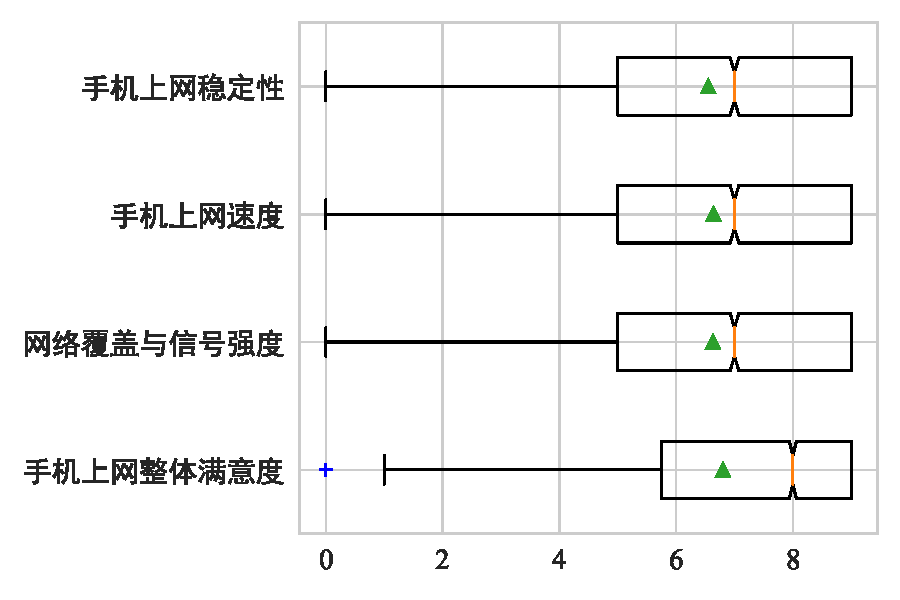
\includegraphics[width=1.0\linewidth]{[附件2][手机上网整体满意度、网络覆盖与信号强度、手机上网速度、手机上网稳定性]评分箱线图.pdf}
			\caption{上网业务用户四项评分箱线图}
			\label{fig:上网业务箱线图}
		\end{minipage}
	\end{figure}
	依据上图结果,我们可以发现用户对于每一业务的四项评分,其分布规律大致一致,但也存在少量异常的数据,为了更清晰地发现各评分之间的散点关系,我们再绘制出语音及上网业务的评分联合分布图,如\textcolor{blue}{\cref{fig:语音业务联合分布图}}、\textcolor{blue}{\cref{fig:上网业务联合分布图}}所示。
	\begin{figure}
		\centering
			\centering
			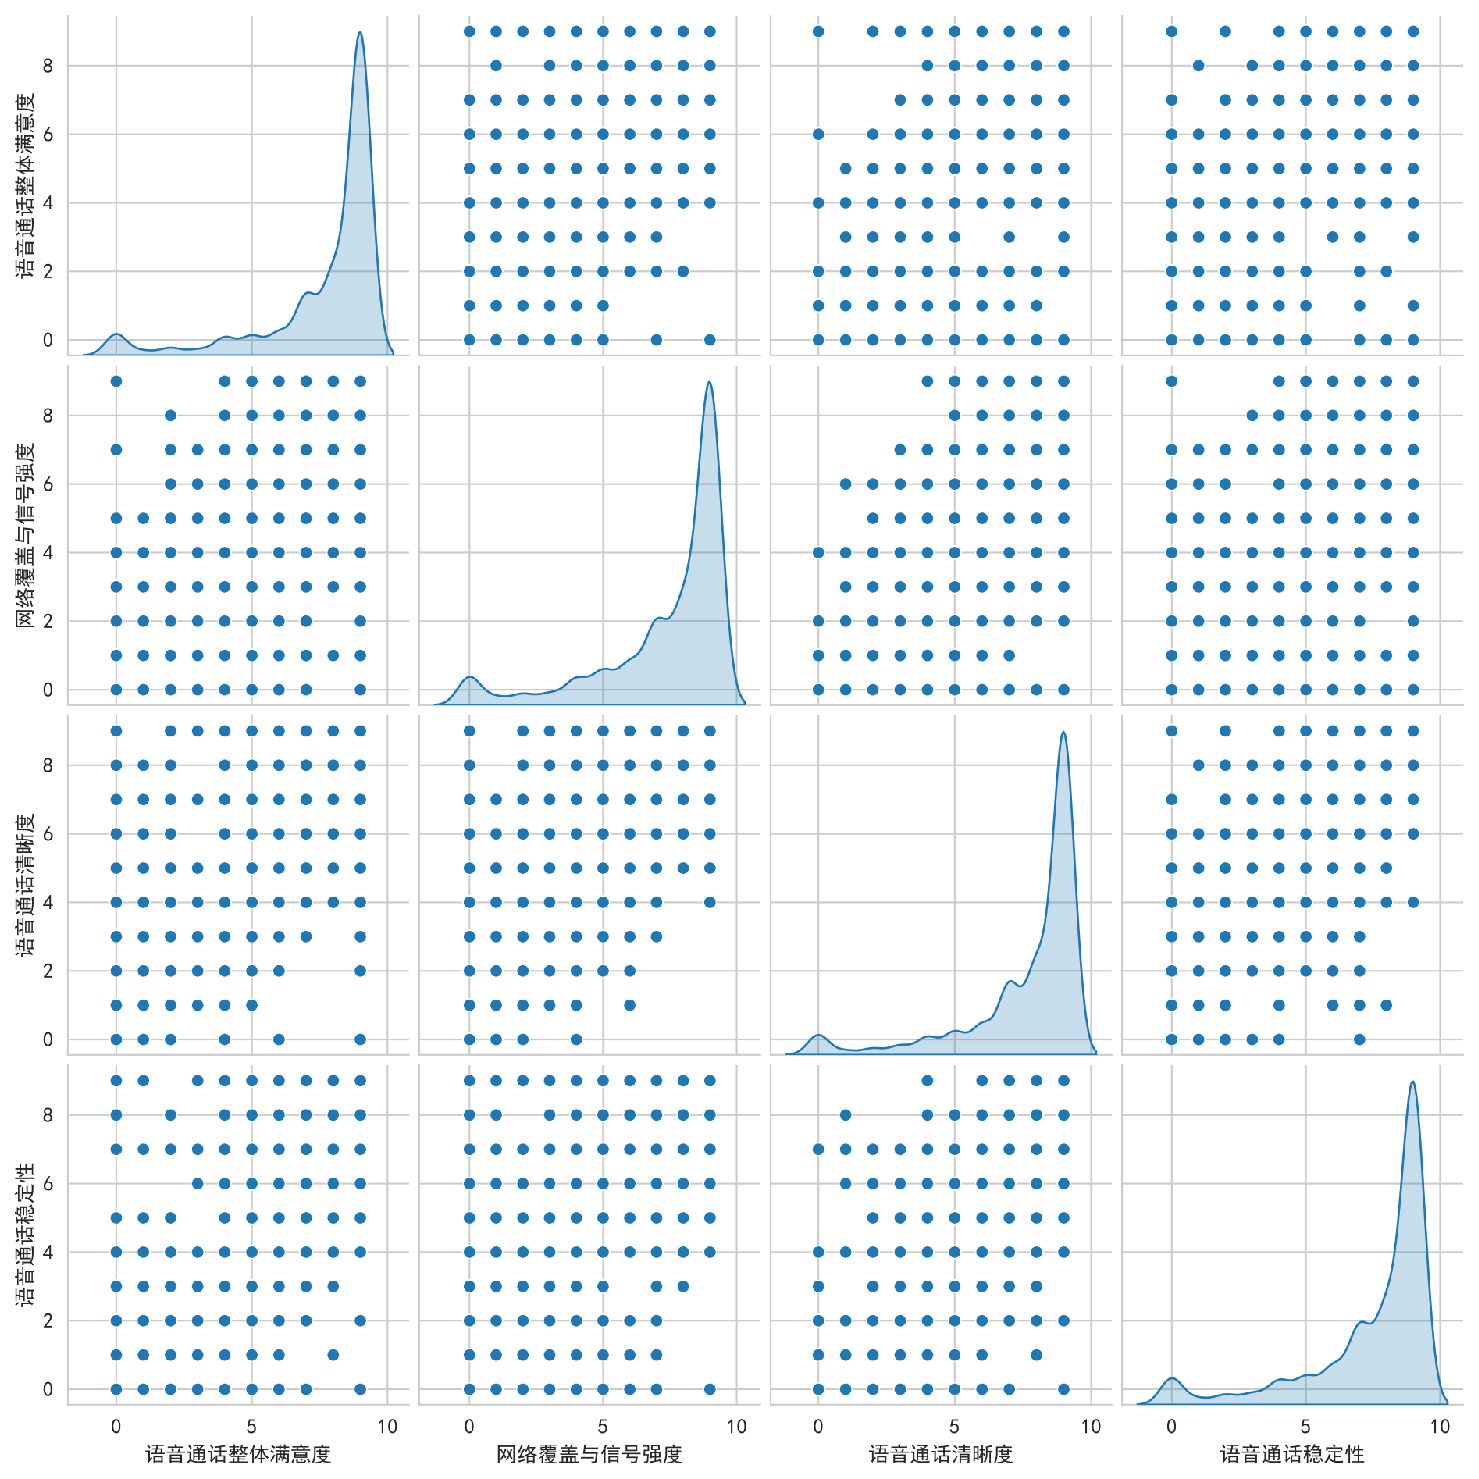
\includegraphics[width=0.6\linewidth]{[附件1][语音通话整体满意度、网络覆盖与信号强度、语音通话清晰度、语音通话稳定性]评分联合分布图_纯图版.pdf}
			\caption{语音业务用户四项评分联合分布图}
			\label{fig:语音业务联合分布图}
	\end{figure}
	\begin{figure}
		\centering
			\centering
			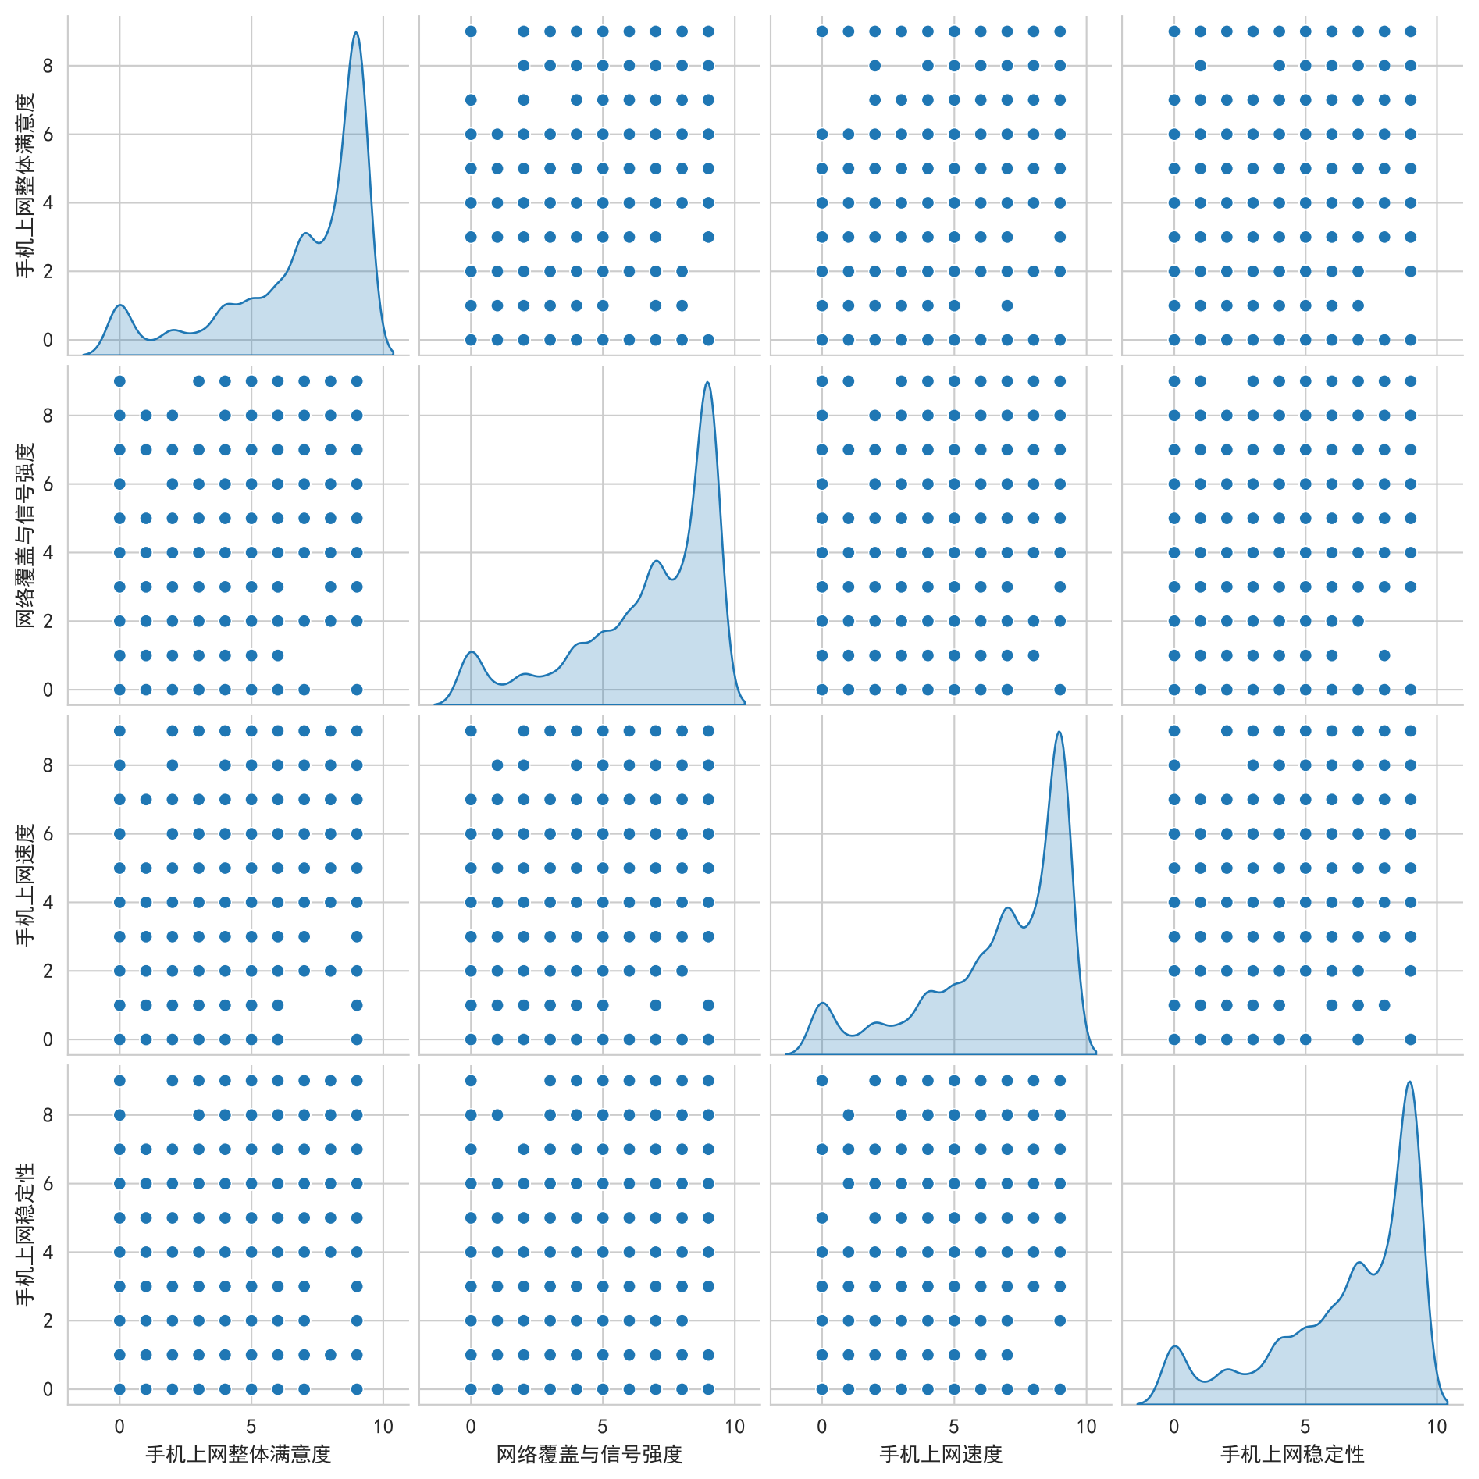
\includegraphics[width=0.6\linewidth]{[附件2][手机上网整体满意度、网络覆盖与信号强度、手机上网速度、手机上网稳定性]评分联合分布图_纯图版.pdf}
			\caption{上网业务用户四项评分联合分布图}
			\label{fig:上网业务联合分布图}
	\end{figure}
	\subsection{多分类模型的建立}
	本文依旧采用初赛使用的六种多分类模型,并对其进行Stacking集成学习。首先多分类基本模型建立理论如下:
	\begin{itemize}
		\item \textbf{随机森林(Random Forest, RF)}是由多棵决策树(Decision Tree)进行组合后对预测结果投票或取均值的一种算法\textcolor{blue}{\cite{prf}}。其有分类和回归两种模型,对于本题,我们选择分类模型。其简要过程如\textcolor{blue}{\cref{fig:RF}}所示,算法伪代码如\textcolor{blue}{Algorithm\ref{RFfunction}}所示。
	
		\scalebox{0.88}{
		\begin{algorithm}[H]
			\label{RFfunction}
			\KwData{数据集$\mathcal{D}$}
			\textbf{function} DTree$\left(\mathcal{D}\right)$\
			
			\eIf{Termination}
			{\textbf{return} $\mathrm{base}\left(g_t\right)$}
			{\textbf{learn} $b\left(x\right)$并且依据$b\left(x\right)$划分$\mathcal{D}$为$\mathcal{D}_C$\
	
			\textbf{build} $G_C \leftarrow$ DTree($\mathcal{D}_C$)\
	
			\textbf{return} $G\left(x\right)=\sum\limits_{C=1}^{C}[\![b\left(x\right)=C]\!]G_C\left(x\right)$}
			
			\textbf{function} RandomForest$\left(\mathcal{D}\right)$\
			
			\For{$t=1,2,3,\cdots,T$}{\textbf{request} 数据集$\tilde{\mathcal{D}}_t \leftarrow$ BoostStrapping$\left(\mathcal{D}\right)$\
			
			\textbf{obtain} DTree $g_t\leftarrow$ DTree$\left(\tilde{\mathcal{D}}_t\right)$\
	
			\textbf{return} $G=$ Uniform$\left(g_t\right)$
			}
			
			\KwResult{随机森林模型$G=\mathrm{Uniform}\left(g_t\right)$}
			\caption{随机森林(RF)}
		\end{algorithm}}
		\begin{figure}[H]
			\centerline{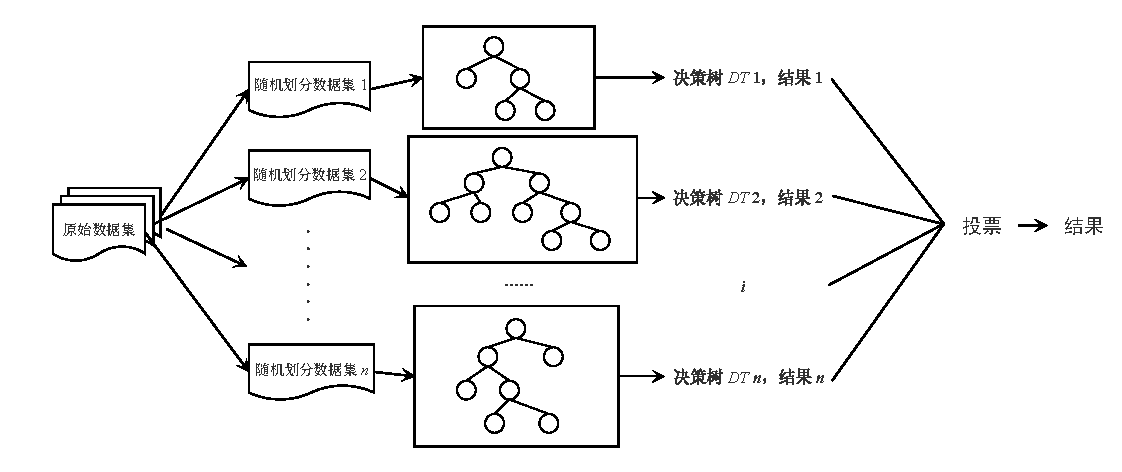
\includegraphics[scale=0.80]{随机森林简图.pdf}}
			\caption{随机森林算法简图}\label{fig:RF}
		\end{figure}
		
		对于单棵决策树而言,本文利用\textbf{CART}算法\textcolor{blue}{\cite{prf}}构建。基尼系数是衡量样本集合纯度的指标,当该值越小时,其纯度也就越高。计算公式如下
		\begin{equation}
			Gini\left( R_i \right)=\sum\limits_{k=1}^{K}\sum\limits_{k\ne k'}P_k P_{k'}=1-\sum\limits_{k=1}^{K}P_k^2 \label{fGini}
		\end{equation}
		其中,$R$为选取出的特征(影响因素),$K$表示在该特征中包含的类别数,$P_k$表示该特征中第$k$类别的出现概率。
	
		由上述分析可知,对于单棵决策树而言,其叶子节点的分裂特征为选择的所有特征中基尼系数最小的特征。
		\item \textbf{极端梯度提升(eXtreme Gradient Boosting, XGBoost)}。XGBoost算法是一种基于树模型的优化模型,其将弱分类器组合,训练出一个较强的分类器。该算法通过多次迭代,生成一个新的树模型用于优化前一个树模型,随着迭代次数的增多,该模型的预测精度也会相应提高\textcolor{blue}{\cite{pxgboost1}}。

		记通过数据处理后的数据集特征为$R\left(x_{ij}\right)_{m\times n}$,表示其包含$m$个用户,$n$个特征,在训练中形成的CART树的集合记为$F=\left\{f\left(x\right)=w_{q\left(x\right)},q:\mathbf{R}^n\to T,w\in \mathbf{R}^T\right\}$,其中$q$为树模型的叶节点决策规划,$T$为某一树模型叶节点数量,$w$为叶节点对应的得分\textcolor{blue}{\cite{pxgboost2}}。对于预测的$y$值,其计算公式为
		\begin{equation}
			\hat{y}=\varphi \left( x_i \right) =\sum\limits_{k=1}^K{f_k\left( x_i \right)} \label{fXGBoostypre}
		\end{equation}
	
		XGBoost算法在每一次迭代过程中会保存前面所学习的模型,会将这些模型加入到新一轮迭代过程中,因此我们记第$i$个模型为预测结果为
		\begin{equation}
			\hat{y}_{i}^{\left(t\right)}=\hat{y}_{i}^{\left(t-1\right)}+f_t\left(x_i\right) \label{fXGBoostyprei}
		\end{equation}
		
		XGBoost算法的目标函数计算公式如下
		\begin{equation}
			L^{\left(t\right)}=\sum\limits_{i=1}^{n}l\left(y_i,\hat{y}_{i}^{\left(t-1\right)}+f_t\left(x_i\right)\right)+\gamma T+\frac{1}{2}\lambda\sum\limits_{j=1}^T{w_j^2}+\mathrm{const} \label{fXGBoostL}
		\end{equation}
		% 其中
		% \begin{equation}
		% 	\Omega\left(f_t\right)=\gamma T+\frac{1}{2}\lambda\sum\limits_{j=1}^T{w_j^2} \label{fXGBoostOmega}
		% \end{equation}
		上述公式中,$l$为模型误差损失,描述在该模型下预测值与实际值之间的出差异损失,$\Omega$为模型叶节点的正则项惩罚系数,$\gamma$与$\lambda$为模型的超参数\textcolor{blue}{\cite{pxgboost2}}。
		通常情况下,我们难以用枚举法得到在模型中所训练出来的树结构,因此这里采用贪婪算法,从单叶子节点开始,通过迭代方法,将其加入到树结构中,从而得到最优解,其计算公式\textcolor{blue}{\cite{pxgboost3}}如下
		\begin{equation}
			\mathcal{L}_{split}=\frac{1}{2}\left[\frac{\left(\sum_{i\in I_L}g_i\right)^2}{\sum_{i\in I_L}h_i+\lambda}+\frac{\left(\sum_{i\in I_R}g_i\right)^2}{\sum_{i\in I_R}h_i+\lambda}-\frac{\left(\sum_{i\in I}g_i\right)^2}{\sum_{i\in I}h_i+\lambda}\right]-\gamma \label{fXGBoostLsplit}
		\end{equation}
		其中$I_j=\left\{i|q\left(x_i\right)=j\right\}$为叶节点$j$上的样本集合\textcolor{blue}{\cite{pxgboost2}},且有
		\begin{equation}
			g_i=\partial_{\hat{y}^{\left(t-1\right)}}l\left(y_i,\hat{y}_i^{\left(t-1\right)}\right)
		\end{equation}
		\begin{equation}
			h_i=\partial_{\hat{y}^{\left(t-1\right)}}^2l\left(y_i,\hat{y}_i^{\left(t-1\right)}\right) \label{xgboosthi}
		\end{equation}
	
		通过上述分析,我们可以得到XGBoost算法简图,如\textcolor{blue}{\cref{fig:XGBoost}}所示。
		\begin{figure}[h!t]
			\centerline{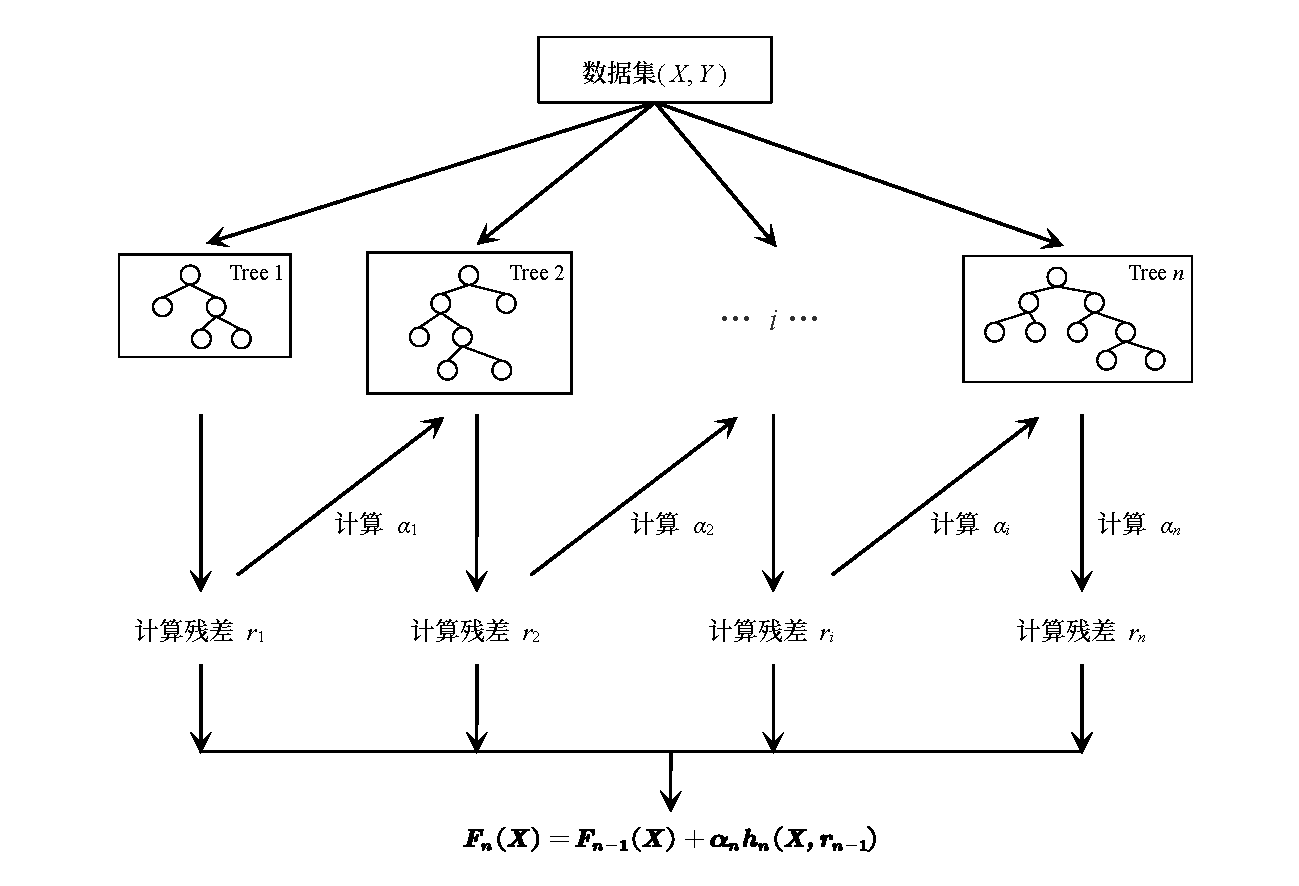
\includegraphics[scale=0.60]{XGBoost简图.pdf}}
			\caption{XGBoost算法简图}\label{fig:XGBoost}
		\end{figure}
		\item \textbf{K-近邻(K Nearest Neighbor, KNN)}。KNN算法的主要思想为:在出现新样本时从现有的训练数据中找到与其相对应的最接近的$K$个样本,并根据最相似的类别出现的样本进行分类。基于多数$K$个样本所属的类别来分辨待分类的数据集所属的类别\textcolor{blue}{\cite{pknn}}。接近度由两点之间的距离函数给出属性空间中的点决定。距离函数通常使用两个点之间的标准欧几里得距离。欧氏距离的计算公式如下
		\begin{equation}
			d(X, Y)=\sqrt{\sum\limits_{i=1}^{n}\left(X_{i}-Y_{i}\right)^{2}} \label{fdistance}
		\end{equation}
		其中$X=\left(x_{1},x_{2},\cdots,x_{m}\right)^{\mathrm{T}}$和$Y=\left(y_{1},y_{2},\cdots,y_{m}\right)^{\mathrm{T}}$表示两个样本列数据,$m$为样本数量。
		
		\item \textbf{支持向量机(Support Vector Machine, SVM)}。SVM建立在结构风险最小原理及Vapnik-Chervonenkis理论基础之上\textcolor{blue}{\cite{psvm}},以有限的数据信息,在数据样本中找出合适区分类别的决策分界面,且保证边界点与分界面尽可能远,即需要再找出合适的边界分界面,该算法示意图如\textcolor{blue}{\cref{fig:svmpicture}}所示。
		\begin{figure}[h!t]
			\centerline{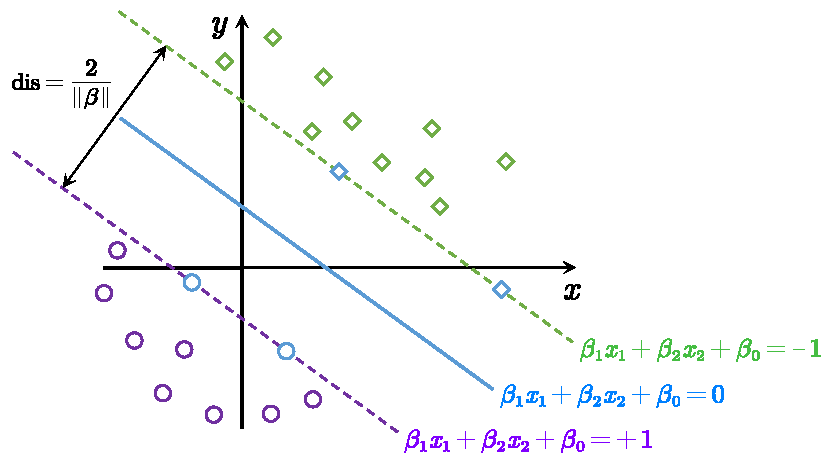
\includegraphics[scale=0.88]{SVM示意图.pdf}}
			\caption{SVM示意图}\label{fig:svmpicture}
		\end{figure}
		而由于SVM多应用于解决二分类问题,且我们需要建立多分类模型,因此需要对其进行相应的改进。本文采用OVR(One Versus Rest)方法,将该问题改进为多个二分类问题\textcolor{blue}{\cite{psvm}}。在模型的训练时,任意将某一类别记为一类,其余类别记为另一类别,依次下去,建立出多分类的SVM模型。而对于核函数的选择,本文选择高斯核函数进行求解,其定义公式如下
		\begin{equation}
			K\left(x_i, x_j\right)=\exp \left(-\frac{\left\|x_i-x_j\right\|^{2}}{2\sigma^{2}}\right)=\exp \left(-\gamma \left\|x_i-x_j\right\|^{2}\right) \label{fgauss}
		\end{equation}
		对于高斯核函数,其可以反映出样本两点之间的相似度大小。当$\sigma$确定后,若两点之间距离越小,则相似度趋近于1;若距离越大,则相似度趋近于0。
		\item \textbf{LightGBM(Light Gradient Boosting Machine)}。LightGBM模型是基于决策树算法构建的一种高效的机器学习算法\textcolor{blue}{\cite{plightgbm}}。其为XGBoost、直方图算法(Histogram)、基于梯度的单边采样(GOSS)算法以及互斥特征捆绑(EFB)算法的结合的一种算法。
		
		\item \textbf{多分类逻辑回归(Multinomial Logistic Regression)}。多分类逻辑回归是基于逻辑回归(Logistic Regression)进行学习的分类模型。对于逻辑回归模型,其属于分类模型,多用于二分类问题。若数据集为$\left(\boldsymbol{A},\boldsymbol{B}\right)=\left(\left(\boldsymbol{a}_1,b_1\right),\left(\boldsymbol{a}_2,b_2\right),\cdots,\left(\boldsymbol{a}_m,b_m\right)\right)^{\mathrm{T}}$,其中$\boldsymbol{a}_i=\left(a_i^1,a_i^2,\cdots,a_i^j\right)$,$a_i^j$为样本$\boldsymbol{a}_i$的第$j$个特征,$\boldsymbol{B}$为因变量标签矩阵,该模型使用Sigmoid函数,同时构建样本$\boldsymbol{a}_i$所属类别的概率,对于标签为$1$的结果,其概率可写为
		\begin{equation}
			P\left(b_i=1\mid \boldsymbol{a}_i,\boldsymbol{\omega}\right)=\frac{1}{1+\mathrm{e}^{-\boldsymbol{a}_ib_i\boldsymbol{\omega}^\mathrm{T}}} \label{fLRp}
		\end{equation}
		其中$\boldsymbol{\omega}=\left(\omega^0,\omega^1,\cdots,\omega^n\right)^\mathrm{T}$为权重向量,即为优化模型的超参数。
		逻辑回归中利用损失函数来评估模型的预测结果与实际值之间的误差,其计算公式如下
		\begin{equation}
			L\left(\boldsymbol{A},\boldsymbol{B},\boldsymbol{\omega}\right)=\frac{1}{m}\sum\limits_{i=1}^{m}\log \left(1+\mathrm{e}^{-\boldsymbol{a}_ib_i \boldsymbol{\omega}^{\mathrm{T}}}\right) \label{fLRl}
		\end{equation}
		而对于$\boldsymbol{\omega}$,常采用梯度下降法来获得模型参数的最优解,其通过
		\begin{equation}
			\boldsymbol{\omega}^{\alpha+1}=\boldsymbol{\omega}^\alpha-\frac{\gamma}{m}\sum\limits_{i=1}^{m}\left(\frac{1}{1+\mathrm{e}^{-\boldsymbol{a}_ib_i \boldsymbol{\omega}^{\mathrm{T}}}}-1\right)\boldsymbol{a}_ib_i \label{fLRw}
		\end{equation}
		进行迭代更新,其中$\gamma$为模型的学习率,当$\left|  \boldsymbol{\omega}^{\alpha}-\boldsymbol{\omega}^{\alpha+1} \right|<\eta$或达到最大迭代次数时,停止训练,输出最终模型,其中$\eta$为人为给定的阈值\textcolor{blue}{\cite{plr}}。
	\end{itemize}

	建立好上述六种多分类模型后,我们依据各模型的预测准确率、平均绝对误差、均方误差,建立Stacking集成学习,将上述模型有目的地进行合理组合,从各模型中学到优点,有利于模型的效果的提升。其基本过程为,首先将已经经过处理的原数据集划分成若干个子集数据,在第一层建立多个模型的融合模型,输入数据,并采用五折交叉验证,获得每个模型的对于因变量标签的预测结果;之后第一层的输出结果作为第二层较弱分类模型的输入数据,第二层单个模型进行训练学习,得到最终预测结果\textcolor{blue}{\cite{pstacking}}。算法示意图如\textcolor{blue}{\cref{fig:StackingPicture}}所示,算法伪代码如\textcolor{blue}{Algorithm\ref{StackingFunciton}}所示。

	\scalebox{0.88}{
	\begin{algorithm}[H]
		\label{StackingFunciton}
		\KwIn{训练集$\mathcal{D}$\

		第一层学习模型$\mathcal{F}_1$,$\mathcal{F}_2$,$\cdots$,$\mathcal{F}_n$\

		第二层学习模型$\mathcal{S}$}
		\For{$t=1,2,3,\cdots,n$}{$h_n=\mathcal{F}_n\left(\mathcal{D}\right)$}
		$\mathcal{D}'=\varnothing$\

		\For{$i=1,2,\cdots,m$}{\For{$t=1,2,\cdots,n$}{$z_{in}=h_n\left(x_i\right)$}
		$\mathcal{D}'=\mathcal{D}'\cup\left(\left(z_{i1},z_{i2},\cdots,z_{in}\right),y_i\right)$}
		$h'=\mathcal{S}\left(D'\right)$

		\KwOut{$\mathcal{H}\left(x\right)=h'\left(h_1\left(x\right),h_2\left(x\right),\cdots,h_n\left(x\right)\right)$}
		\caption{Stacking集成学习}
	\end{algorithm}}
	\begin{figure}[H]
		\centerline{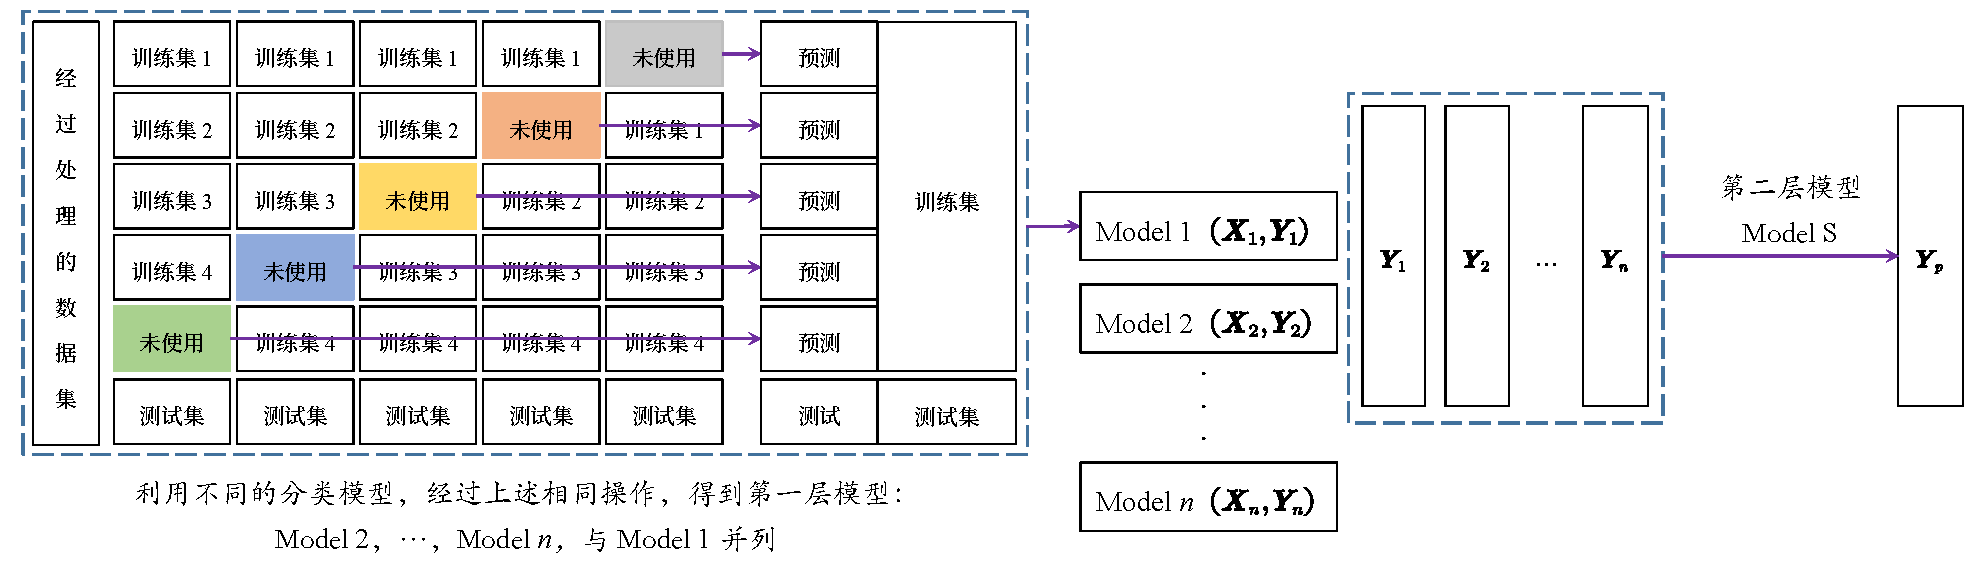
\includegraphics[scale=0.56]{Stacking示意图.pdf}}
		\caption{Stacking集成学习示意图}\label{fig:StackingPicture}
	\end{figure}
	\subsubsection{语音业务求解}



	以箱线图所示,用户评分,划分高分组与低分组。
	思路:绘制评分联合分布图,观察用户行为。得出异常点,初始确定用户错评,乱评等不合理行为的依据。
	语音、上网业务各四项评分,联合确定高分组及低分组,筛选出高分及低分组,对数据进行可视化、描述性分析,得出高分组及低分组的特征。综合之前的初步确定,则得出用户错评的依据,对数据进行综合筛选,对筛选出的数据与原始数据进行对比,确定其合理性。
	重新学习、预测!分析合理性。

	非技术性报告
	\section{模型的评价与推广}
	\subsection{模型的评价}
	\begin{itemize}
		\item \textbf{模型的优点}:
			\begin{enumerate}
				\item 对数据进行综合处理,层次清晰,模型具有一定解释性;
				\item 数据标准化,避免量纲不一造成的偏向学习影响的情况;
				\item 特征筛选,减少不重要性因素占比,减少数据维度,提升模型学习效率,一定程度上避免数据噪声,适当降低模型复杂度,使模型高效化,防止过拟合;
				\item 特征构造,由原数据构造出新数据特征,适当增多数据维度,防止欠拟合;
				\item 综合熵权法、灰色关联度分析及随机森林量化影响程度,避免局部最优;
				\item 对各模型进行参数调优,尽可能提高模型的多方面能力;
				\item 加入正则化方法,一定程度上也可防止过拟合;
				\item 交叉验证,更好地利用数据集,减少数据浪费,提高模型的泛化能力,验证模型的稳健性,防止过拟合情况的发生;
				\item 模型设置任意随机种子,在保证划分训练集及测试集的一般性、随机性的同时,确保可重复性的结果,方便后续处理;
				\item 通过主成分分析及随机森林进行特征选择,保证客观性;
				\item 多模型Stacking集成学习,更好地利用已有数据,多方面学习数据中内在联系,结合多个模型优良方面,避免陷入局部最优,对数据有更好的把控能力,提升模型的泛化能力、提高预测准确率、提高模型稳健性、鲁棒性,同时减小预测误差,且对异常值有一定识别能力。
			\end{enumerate}
		\item \textbf{模型的缺点}:
			\begin{enumerate}
				\item 模型对于小样本分类的识别能力较差,难以对这些用户进行深入分析;
				\item 模型对于预测主观性评分,难以提供完全一致的评分结果;
				\item Stacking在构造时,有一定复杂度,对基模型的要求较高;
				\item 对于部分评分,特征构造出的因素有一定局限性;
				\item 用户评分为主观性结果,本文大多模型选用客观性较强的模型进行解决,对数据利用有一定失真。
			\end{enumerate}
		\newpage
		\item \textbf{模型的改进}:
			\begin{enumerate}
				\item 在收集数据时,问卷设计需要更加合理化,多方面考虑其余未考虑到的影响因素对用户评分的影响;
				\item 在允许条件下获得更多训练样本;
				\item 对各模型可以选用非完全一致的特征,提升各模型的独特性,有目的地进行选择,减少学习的数据维度,加快模型收敛速度,使得模型学习高效化,结果准确化;
				\item 适当增加或减少数据维度,建立复杂度适中的模型;
				\item 对不平衡的多分类,可以采用“下采样”或“上采样”方法,使得分类平衡,但需要更多的数据集;
				\item 可适当增加基模型个数,并提高对基模型的筛选要求;
				\item 对主观性评分,可以建立主客观相结合的模型,从而优化模型各项指标。
			\end{enumerate}
	\end{itemize}
	\subsection{模型的推广}
	机器学习可利用现有的数据集进行有目的的训练,在此基础上预测分类标签下人为难以确定的结果,极大方便了当今对复杂数据的处理;多种机器学习相互结合,利用Stacking集成学习的方法,可以有效提高模型各方面能力,减少判断错误的情况。针对小部分样本的学习,需要更容易区分类别的特征进行学习,以及利用特征工程等方法进行解决。对于机器学习模型,我们可以作出其可视化图像,观察到模型的各项指标不易发现的问题,如欠拟合、过拟合等情况,我们可以依据模型效果评估可视化来对模型进行一定的调优。本文是以移动用户对业务的评分为基础,我们运用了多种机器学习的模型,再结合Stacking进行集成学习,可以发现模型的效果较优,对主观性评分模型有较好把控能力。利用该模型,可以根据用户对某些影响因素的情况,预测用户对于这项业务的满意程度,再结合相关描述性信息,有的放矢地解决用户遇到的问题,提升客户的满意程度,提升产品的服务质量,从而为业务创造更多价值。该模型在一定程度上虽有一定欠缺,但不仅仅可用于该领域的评分,也可用于其余领域,如用户对于某一产品的评价预测,根据用户评价,改善产品质量,提升经济效益,实现双赢。

	\newpage
	\phantomsection
	\addcontentsline{toc}{section}{\textbf{参考文献}}
	\begin{spacing}{1.08}
	\begin{thebibliography}{99}
	\bibitem{pstandard}CSDN.【数据预处理】sklearn实现数据预处理(归一化、标准化)[EB/OL].
	
	\url{https://blog.csdn.net/weixin_44109827/article/details/124786873}.

	\bibitem{ppearson1}肖杨,李亚,王海瑞,常梦容.基于皮尔逊相关系数的滚动轴承混合域特征选择方法[J].化工自动化及仪表,2022,49(03):308-315.DOI:10.20030/j.cnki.1000-3932.202203009.

	\bibitem{prf}饶雷,冉军,陶建权,胡号朋,吴沁,熊圣新.基于随机森林的海上风电机组发电机轴承异常状态监测方法[J].船舶工程,2022,44(S2):27-31.DOI:10.13788/j.cnki.cbgc.2022.S2.06.

	\bibitem{pxgboost1}陈振宇,刘金波,李晨,季晓慧,李大鹏,黄运豪,狄方春,高兴宇,徐立中.基于LSTM与XGBoost组合模型的超短期电力负荷预测[J].电网技术,2020,44(02):614-620.DOI:10.13335/j.1000-3673.pst.2019.1566.

	\bibitem{pxgboost2}杨贵军,徐雪,赵富强.基于XGBoost算法的用户评分预测模型及应用[J].数据分析与知识发现,2019,3(01):118-126.

	\bibitem{pxgboost3}Tianqi Chen and Carlos Guestrin. 2016. XGBoost: A Scalable Tree Boosting System. In Proceedings of the 22nd ACM SIGKDD International Conference on Knowledge Discovery and Data Mining (KDD '16). Association for Computing Machinery, New York, NY, USA, 785–794. \url{https://doi.org/10.1145/2939672.2939785}.

	\bibitem{pknn}张著英,黄玉龙,王翰虎.一个高效的KNN分类算法[J].计算机科学,2008(03):170-172.

	\bibitem{psvm}汪海燕,黎建辉,杨风雷.支持向量机理论及算法研究综述[J].计算机应用研究,2014,31(05):1281-1286.

	\bibitem{plightgbm}马晓君,沙靖岚,牛雪琪.基于LightGBM算法的P2P项目信用评级模型的设计及应用[J].数量经济技术经济研究,2018,35(05):144-160.DOI:10.13653/j.cnki.jqte.20180503.001.

	\bibitem{plr}唐敏,张宇浩,邓国强.高效的非交互式隐私保护逻辑回归模型[J/OL].计算机工程:1-11[2023-01-04].DOI:10.19678/j.issn.1000-3428.0065549.

	\bibitem{pstacking}史佳琪,张建华.基于多模型融合Stacking集成学习方式的负荷预测方法[J].中国电机工程学报,2019,39(14):4032-4042.DOI:10.13334/j.0258-8013.pcsee.181510.

	\end{thebibliography}
	\end{spacing}
	\newpage

	\phantomsection
	\addcontentsline{toc}{section}{\textbf{附\hspace{2pc}录}}

	% \appendix
	% \ctexset{section={format={\zihao{-4}\heiti\raggedright}}}
	\begin{center}
		\heiti\zihao{4} 附\hspace{2pc}录
	\end{center}

% \phantomsection
% \addcontentsline{toc}{subsection}{[A]图示}
% 	% \section*{[A]图表}
	\noindent{\heiti [A]图表}

\newpage
% \phantomsection
% \addcontentsline{toc}{subsection}{[B]支撑文件列表}
% 	% \section*{[B]支撑文件列表}
	\noindent{\heiti [B]支撑文件列表}
	~\\

	支撑文件列表如下(列表中不包含原始数据集):
	% Table generated by Excel2LaTeX from sheet 'Sheet2'
	\begin{table}[htbp]
	\centering
	\scalebox{0.88}{
	  \begin{tabular}{cc}
	  \toprule
	  \textbf{文件(夹)名} & \textbf{描述} \\
	  \midrule
	  result.xlsx & 用户评分预测结果 \\
	  所有量化结果.xlsx & 问题一量化结果 \\
	  模型参数.xlsx & 各个模型评估参数以及模型选择依据 \\
	  语音业务词云.txt & 语音业务词云图文本内容 \\
	  上网业务词云.txt & 上网业务词云图文本内容 \\
	  语音业务数据分析.ipynb & 语音业务分析Jupyter文件 \\
	  上网业务数据分析.ipynb & 上网业务分析Jupyter文件 \\
	  语音业务数据分析.html & 语音业务分析运行结果 \\
	  上网业务数据分析.html & 上网业务分析运行结果 \\
	  bg.jpg & 词语底图 \\
	  figuresNightingaleRoseDiagramF.py & 原始数据用户评分南丁格尔玫瑰图程序 \\
	  figuresNightingaleRoseDiagramP.py & 预测数据用户评分南丁格尔玫瑰图程序 \\
	  figuresOne & 语音业务所有图示文件夹 \\
	  figuresTwo & 上网业务所有图示文件夹 \\
	  figuresNightingaleRoseDiagramF & 原始数据用户评分南丁格尔玫瑰图示(八项评分) \\
	  figuresNightingaleRoseDiagramP & 预测数据用户评分南丁格尔玫瑰图示(八项评分) \\
	  \bottomrule
	  \end{tabular}}
  	\end{table}
  
\newpage
% \phantomsection
% \addcontentsline{toc}{subsection}{[C]使用的软件、环境}
	% \section*{[C]使用的软件、环境}
	\noindent{\heiti [C]使用的软件、环境}
	~\\

	为解决该问题,我们所使用的主要软件有:
	\begin{itemize}
		\item TeX Live 2022
		\item Visual Studio Code 1.76.1
		\item WPS Office 2022冬季更新(13703)
		\item Python 3.10.4
		\item Pycharm Professional 2022.3
	\end{itemize}
	
	Python环境下所用使用到的库及其版本如下:
\begin{table}[htbp]
	\centering
	\setlength{\aboverulesep}{0pt}
	\setlength{\belowrulesep}{0pt}
	\scalebox{0.88}{
	  \begin{tabular}{cc||cc}
	  \toprule
	  \textbf{库} & \textbf{版本} & \textbf{库} & \textbf{版本} \\
	  \midrule
	  copy  & 内置库   & missingno & 0.5.1 \\
	  jieba & 0.42.1 & mlxtend & 0.20.2 \\
	  jupyter & 1.0.0 & numpy & 1.22.4+mkl \\
	  jupyter-client & 7.3.1 & openpyxl & 3.0.10 \\
	  jupyter-console & 6.4.3 & pandas & 1.4.2 \\
	  jupyter-contrib-core & 0.4.0 & pyecharts & 1.9.1 \\
	  jupyter-contrib-nbextensions & 0.5.1 & scikit-learn & 0.22.2.post1 \\
	  jupyter-core & 4.10.0 & seaborn & 0.11.2 \\
	  jupyter-highlight-selected-word & 0.2.0 & sklearn & 0.0  \\
	  jupyterlab-pygments & 0.2.2 & snapshot\_phantomjs & 0.0.3 \\
	  jupyterlab-widgets & 1.1.0 & warnings & 内置库 \\
	  jupyter-latex-envs & 1.4.6 & wordcloud & 1.8.1 \\
	  jupyter-nbextensions-configurator & 0.5.0 & xgboost & 1.6.1 \\
	  matplotlib & 3.5.2 & yellowbrick & 1.4 \\
	  \bottomrule
	  \end{tabular}}
\end{table}

\newpage
% \phantomsection
% \addcontentsline{toc}{subsection}{[D]问题解决源程序}
	% \section*{[D]问题解决源程序}
\noindent{\heiti [D]问题解决源程序}

% \phantomsection
% \addcontentsline{toc}{subsubsection}{D.1 语音业务分析代码[针对附件1与附件3]}
\textbf{D.1 语音业务分析代码[针对附件1与附件3]}
\begin{python}
\end{python}
\newpage
% \phantomsection
% \addcontentsline{toc}{subsubsection}{D.2 上网业务分析代码[针对附件2与附件4]}
\textbf{D.2 上网业务分析代码[针对附件2与附件4]}
\begin{python}
\end{python}
\newpage
% \phantomsection
% \addcontentsline{toc}{subsubsection}{D.3 原始数据用户评分南丁格尔玫瑰图示}
\textbf{D.3 原始数据用户评分南丁格尔玫瑰图示}
\begin{python}
\end{python}
\newpage
% \phantomsection
% \addcontentsline{toc}{subsubsection}{D.4 预测数据用户评分南丁格尔玫瑰图示}
\textbf{D.4 预测数据用户评分南丁格尔玫瑰图示}
\begin{python}
\end{python}
\end{document}